\documentclass[main-ap-physics.tex]{subfiles}
\usetikzlibrary{decorations.markings}

\begin{document}

\begin{example}
    \textit{Adding Vectors Using Analytical Methods}\\
    Add the vector \textbf{A} to the vector \textbf{B} shown in Figure \ref{cBsaWa}, using perpendicular components along the $x$- and $y$-axes. The $x$- and $y$-axes are along the east–west and north–south directions, respectively. Vector \textbf{A} represents the first leg of a walk in which a person walks \SI{53.0}{m} in a direction \ang{20.0} north of east. Vector \textbf{B} represents the second leg, a displacement of \SI{34.0}{m} in a direction \ang{63.0} north of east.
\end{example}

\begin{center}
    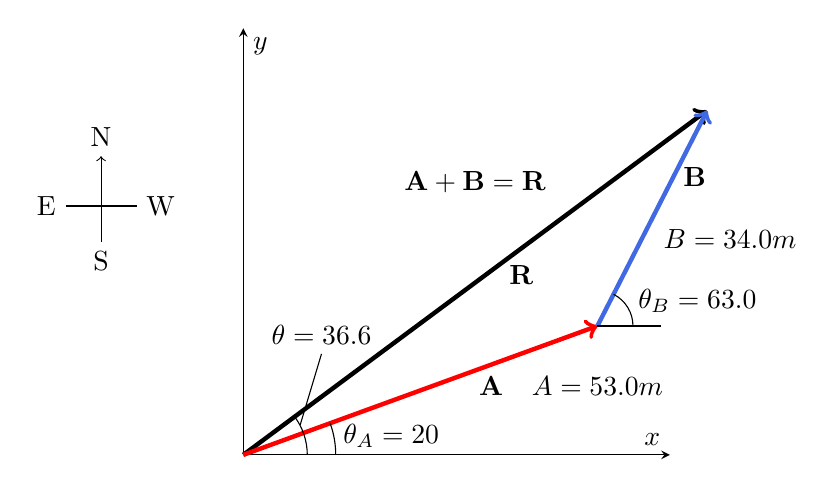
\begin{tikzpicture}
        \begin{axis}[width=7cm,height=7cm,
            axis lines=center,
            xmin=0,xmax=60,
            ymin=0,ymax=60,
            ticks=none,
            clip=false,
            xlabel=$x$,
            ylabel=$y$
        ]
        \coordinate (R) at ({81.2*cos(36.6)},{81.2*sin(36.6)});
        \coordinate (A) at ({53*cos(20)},{53*sin(20)});
        \coordinate (B) at ({34*cos(63)},{34*sin(63)});
        \draw[ultra thick,->] (0,0) -- (R) node[below=2pt,pos=0.6] {\textbf{R}} node[above=1cm,pos=0.5] {$\textbf{A} + \textbf{B} = \textbf{R}$};
        \draw[ultra thick,->,red] (0,0) -- (A) node[below,pos=0.7,black] {\textbf{A}} node[below=5mm,black] {$A = \SI{53.0}{m}$};
        \draw[ultra thick,->,RoyalBlue] (A) -- ++(B) node[below right=-1mm,pos=0.75,black] {\textbf{B}} node[below right,pos=0.5,black] {$B = \SI{34.0}{m}$};
        \draw (9,0) arc (0:36.6:9);
        \draw (13,0) arc (0:20:13) node[right,pos=0.6] {$\theta_{\text{A}} = \ang{20}$};
        \draw (8,4.2) -- ++(3,10) node[above] {$\theta = \ang{36.6}$};
        \begin{scope}[shift={(-20,30)}]
            \draw[->] (0,0) node[below] {S} -- ++(0,12) node[above] {N};
            \draw (-5,5) node[left] {E} -- ++(10,0) node [right] {W};
        \end{scope}
        \draw (A) -- ++(9,0);
        \draw ({53*cos(20) + 5},{53*sin(20)}) arc (0:63:5) node[right=2pt,pos=0.7] {$\theta_{\text{B}} = \ang{63.0}$};
        \end{axis}
    \end{tikzpicture}
    \captionsetup{type=figure,margin=1in,font=scriptsize}
    \captionof{figure}{Vector \textbf{A} has magnitude \SI{53.0}{m} and direction \ang{20.0} north of the $x$-axis. Vector \textbf{B} has magnitude \SI{34.0}{m} and direction \ang{63.0} north of the $x$-axis. You can use analytical methods to determine the magnitude and direction of \textbf{R}.}
\label{cBsaWa}
\end{center}

\Solution \textbf{Strategy}: The components of \textbf{A} and \textbf{B} along the $x$- and $y$-axes represent walking due east and due north to get to the same ending point. Once found, they are combined to produce the resultant.

\vspace{1em}

Following the method outlined above, we first find the components of \textbf{A} and \textbf{B} along the $x$- and $y$-axes. Note that $A = \SI{53.0}{m}$, $\theta_{\text{A}} = \ang{20.0}$, $B = \SI{34.0}{m}$, and $\theta_{\text{B}} = \ang{63.0}$. We find the $x$-components by using $A_x = A \cos{\theta}$, which gives

\begin{equation*}
    A_x = A \cos{\theta_{\text{A}}} = \left(\SI{53.0}{m}\right) \left(\cos{\ang{20.0}}\right) = \left(\SI{53.0}{m}\right) \left(0.940\right) = \SI{49.8}{m}
\end{equation*}

and

\begin{equation*}
    B_x = B\cos{\theta_{\text{B}}} = \left(\SI{34.0}{m}\right) \left(\cos{\ang{63.0}}\right) = \left(\SI{34.0}{m}\right) \left(0.454\right) = \SI{15.4}{m}
\end{equation*}

Similarly, the $y$-components are found using $A_y = A \sin{\theta_{\text{A}}}$:

\begin{equation*}
    A_y = A \sin{\theta_{\text{A}}} = \left(\SI{53.0}{m}\right) \left(\sin{\ang{20.0}}\right) = \left(\SI{53.0}{m}\right) \left(0.342\right) = \SI{18.1}{m}
\end{equation*}

and

\begin{equation*}
    B_y = B\cos{\theta_{\text{B}}} = \left(\SI{34.0}{m}\right) \left(\sin{\ang{63.0}}\right) = \left(\SI{34.0}{m}\right) \left(0.891\right) = \SI{30.3}{m}
\end{equation*}

The $x$- and $y$-components of the resultant are thus

\begin{equation*}
    R_x = A_x + B_x = \SI{49.8}{m} + \SI{15.4}{m} = \SI{65.2}{m}
\end{equation*}

and 

\begin{equation*}
    R_y = A_y + B_y = \SI{18.1}{m} + \SI{30.3}{m} = \SI{48.4}{m}
\end{equation*}

Now we can find the magnitude of the resultant by using the Pythagorean theorem:

\begin{equation*}
    R = \sqrt{R_x^2 + R_y^2} = \sqrt{\left(\SI{65.2}{m}\right)^2 + \left(\SI{48.4}{m}\right)^2} = 
\end{equation*}

so that 

\begin{equation*}
    R = \SI{81.2}{m}
\end{equation*}

Finally, we find the direction of the resultant:

\begin{equation*}
    \theta = \tan^{-1}\left(\frac{R_y}{R_x}\right) = \tan^{-1}\left(\frac{48.4}{65.2}\right) 
\end{equation*}

Thus,

\begin{equation*}
    \theta = \tan^{-1}\left(0.742\right) = \ang{36.6}
\end{equation*}

\begin{center}
    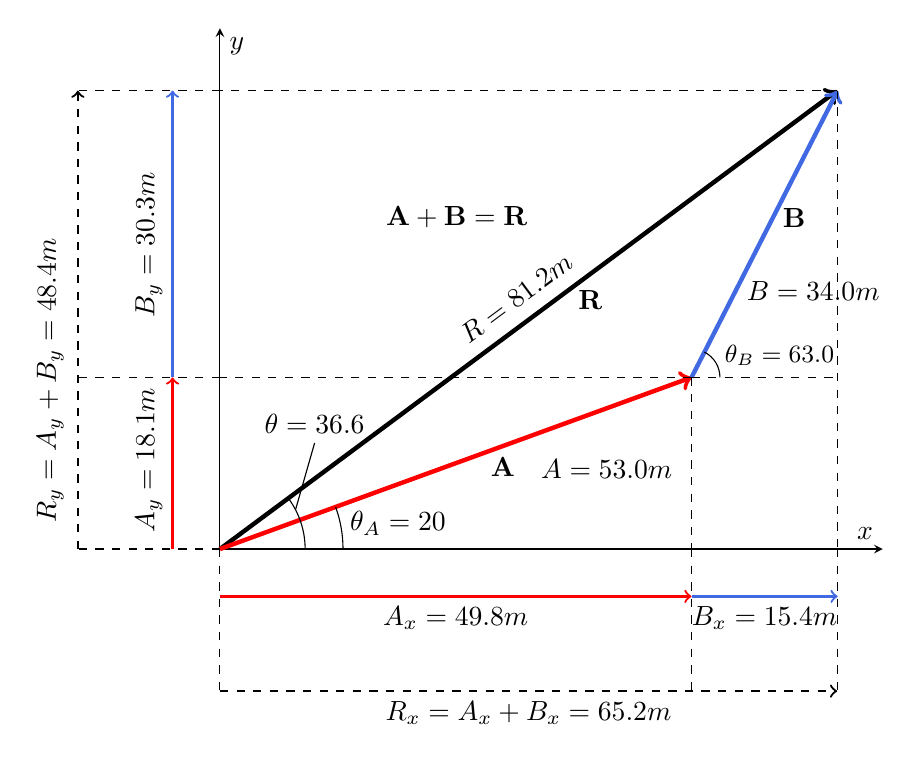
\begin{tikzpicture}
        \begin{axis}[width=10cm,height=10cm,
            axis lines=center,
            xmin=0,xmax=70,
            ymin=0,ymax=55,
            ticks=none,
            clip=false,
            xlabel=$x$,
            ylabel=$y$,
            axis equal image
        ]
        \coordinate (R) at ({81.2*cos(36.6)},{81.2*sin(36.6)});
        \coordinate (Rx) at ({81.2*cos(36.6)},0);
        \coordinate (Ry) at (0,{81.2*sin(36.6)});
        \coordinate (A) at ({53*cos(20)},{53*sin(20)});
        \coordinate (Ax) at ({53*cos(20)},0);
        \coordinate (Ay) at (0,{53*sin(20)});
        \coordinate (B) at ({34*cos(63)},{34*sin(63)});
        \coordinate (Bx) at ({34*cos(63)},0);
        \coordinate (By) at (0,{34*sin(63)});
        
        \draw[ultra thick,->] (0,0) -- (R) node[below=2pt,pos=0.6] {\textbf{R}} node[above=2pt,pos=0.5,rotate=36.6] {$R = \SI{81.2}{m}$};
        \node at (25,35) {$\textbf{A} + \textbf{B} = \textbf{R}$};
        \draw[ultra thick,->,red] (0,0) -- (A) node[below,pos=0.6,black] {\textbf{A}} node[below=5mm,black,pos=0.82] {$A = \SI{53.0}{m}$};
        \draw[ultra thick,->,RoyalBlue] (A) -- ++(B) node[below right=-1mm,pos=0.6,black] {\textbf{B}} node[right,pos=0.3,black] {$B = \SI{34.0}{m}$};
        
        \draw[dashed] (R) -- ++({-81.2*cos(36.6)},0);
        \draw[dashed] (A) -- ++({-53*cos(20)},0);
        \draw[thick,red,->] (-5,0) -- ++(Ay) node[left=3mm,black,rotate=90] {$A_y = \SI{18.1}{m}$};
        \draw[thick,RoyalBlue,->] (-5,{53*sin(20)}) -- ++(By) node[left=3mm,pos=0.75,black,rotate=90] {$B_y = \SI{30.3}{m}$};
        \draw[dashed] (0,{53*sin(20)+34*sin(63)}) -- ++(-15,0);
        \draw[dashed] (0,{53*sin(20)}) -- ++(-15,0);
        \draw[dashed] (0,0) -- ++(-15,0);
        
        \draw[thick,dashed,->] (-15,0) -- ++(Ry) node[left=3.5mm,pos=0.7,rotate=90] {$R_y = A_y + B_y = \SI{48.4}{m}$};
        
        \draw[dashed] (R) -- ++(0,{-81.2*sin(36.6)});
        \draw[dashed] (A) -- ++(0,{-53*sin(20)});
        \draw[thick,red,->] (0,-5) -- ++(Ax) node[below,black,pos=0.5] {$A_x = \SI{49.8}{m}$};
        \draw[thick,RoyalBlue,->] ({53*cos(20)},-5) -- ++(Bx) node[below,black,pos=0.5] {$B_x = \SI{15.4}{m}$};
        \draw[dashed] (0,0) -- ++(0,-15);
        \draw[dashed] ({53*cos(20)+34*cos(63)},0) -- ++(0,-15);
        \draw[dashed] ({53*cos(20)},0) -- ++(0,-15);
        \draw[thick,dashed,->] (0,-15) -- ++(Rx) node[below,pos=0.5] {$R_x = A_x + B_x = \SI{65.2}{m}$};
        \draw (9,0) arc (0:36.6:9);
        \draw (13,0) arc (0:20:13) node[right,pos=0.6] {$\theta_{\text{A}} = \ang{20}$};
        \draw (8,4.2) -- ++(2,7) node[above] {$\theta = \ang{36.6}$};

        \draw[dashed] (A) -- ++(Bx);
        \draw ({53*cos(20) + 3},{53*sin(20)}) arc (0:63:3) node[right=2pt,pos=0.8] {\small $\theta_{\text{B}} = \ang{63.0}$};
        \end{axis}
    \end{tikzpicture}
    \captionsetup{type=figure,margin=1in,font=scriptsize}
    \captionof{figure}{Using analytical methods, we see that the magnitude of \textbf{R} is \SI{81.2}{m} and its direction is \ang{36.6} north of east.}
    \label{QVly9l}
\end{center}

\textbf{Discussion}: This example illustrates the addition of vectors using perpendicular components. Vector subtraction using perpendicular components is very similar--it is just the addition of a negative vector.

\vspace{1em}

Subtraction of vectors is accomplished by the addition of a negative vector. That is, $\textbf{A}-\textbf{B} \equiv \textbf{A}+\left(-\textbf{B}\right)$. Thus, \textit{the method for the subtraction of vectors using perpendicular components is identical to that for addition}. The components of $-\textbf{B}$ are the negatives of the components of \textbf{B}. The $x$- and $y$-components of the resultant  $\textbf{A} - \textbf{B} = \textbf{R}$ are thus

\begin{equation*}
    R_x = A_x + \left(-B_x\right)
\end{equation*}

\begin{equation*}
    R_y = A_y + \left(-B_y\right)
\end{equation*}

and the rest of the method outlined above is identical to that for addition. (See Figure \ref{g2pI0f}.)

\endsolution    

Analyzing vectors using perpendicular components is very useful in many areas of physics, because perpendicular quantities are often independent of one another. The next module, ``Projectile Motion,'' is one of many in which using perpendicular components helps make the picture clear and simplifies the physics.

\begin{center}
    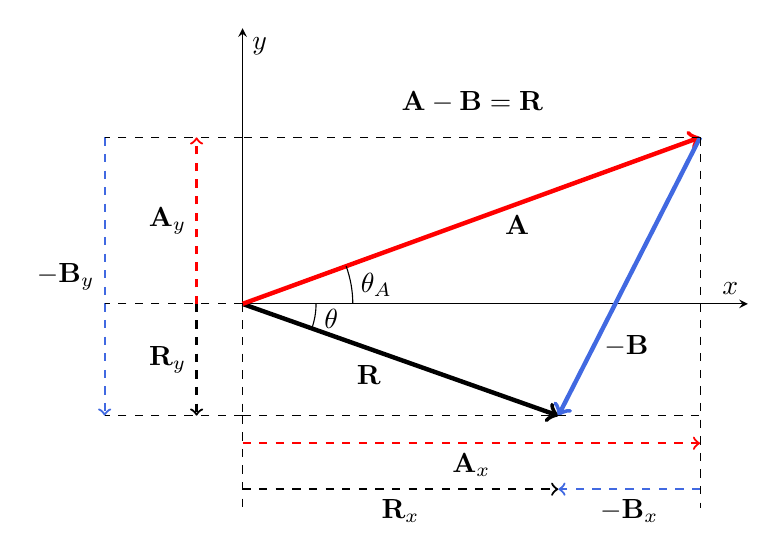
\begin{tikzpicture}
        \begin{axis}[width=8cm,height=8cm,
            axis lines=center,
            xmin=0,xmax=55,
            ymin=0,ymax=30,
            ticks=none,
            clip=false,
            xlabel=$x$,
            ylabel=$y$,
            axis equal image
        ]
        \coordinate (A) at ({53*cos(20)},{53*sin(20)});
        \coordinate (Ax) at ({53*cos(20)},0);
        \coordinate (Ay) at (0,{53*sin(20)});
        \coordinate (B) at ({-34*cos(63)},{-34*sin(63)});
        \coordinate (Bx) at ({-34*cos(63)},0);
        \coordinate (By) at (0,{-34*sin(63)});
        \coordinate (R) at ({53*cos(20)-34*cos(63)},{53*sin(20)-34*sin(63)});
        \coordinate (Ry) at (0,{53*sin(20)-34*sin(63)});
        \coordinate (Rx) at ({53*cos(20)-34*cos(63)},0);
        
        \draw[ultra thick,->] (0,0) -- (R) node[below=2pt,pos=0.4] {\textbf{R}};
        \node at (25,22) {$\textbf{A} - \textbf{B} = \textbf{R}$};
        \draw[ultra thick,->,red] (0,0) -- (A) node[below,pos=0.6,black] {\textbf{A}};
        \draw[ultra thick,->,RoyalBlue] (A) -- ++(B) node[below right=-1mm,pos=0.7,black] {$-\textbf{B}$};
        
        \draw[dashed] (A) -- ++({-53*cos(20)},0);
        
        \draw[thick,dashed,red,->] (-5,0) -- ++(Ay) node[left,black,pos=0.5] {$\textbf{A}_y$};
        \draw[thick,dashed,RoyalBlue,->] (-15,{53*sin(20)}) -- ++(By) node[left,pos=0.5,black] {$-\textbf{B}_y$};
        \draw[thick,dashed,->] (-5,0) -- ++(Ry) node[left,pos=0.5] {$\textbf{R}_y$};

        \draw[dashed] (Ay) -- ++(-15,0);
        \draw[dashed] (A) -- ++(By) -- ++(0,-10);
        \draw[dashed] (0,0) -- ++(Ry);
        \draw[dashed] (Ry) -- ++(-15,0);
        \draw[dashed] (Ry) -- ++(Ax);
        \draw[dashed] (0,0) -- ++(-15,0);
        \draw[dashed] (Ry) -- ++(0,-10);
        \draw[red,thick,dashed,->] (0,{53*sin(20)-34*sin(63)-3}) -- ++(Ax) node[pos=0.5,black,below] {$\textbf{A}_x$};
        \draw[thick,dashed,->] (0,{53*sin(20)-34*sin(63)-8}) -- ++(Rx) node[below,pos=0.5] {$\textbf{R}_x$};
        \draw[thick,RoyalBlue,dashed,->] ({53*cos(20)},{53*sin(20)-34*sin(63)-8}) -- ++(Bx) node[below,pos=0.5,black] {$-\textbf{B}_x$};

        \draw (8,0) arc (0:-19.5:8) node[right,pos=0.6] {$\theta$};
        \draw (12,0) arc (0:20:12) node[right,pos=0.5] {$\theta_{\text{A}}$};
        
        \end{axis}
    \end{tikzpicture}
    \captionsetup{type=figure,margin=1in,font=scriptsize}
    \captionof{figure}{The subtraction of the two vectors shown in Figure \ref{i2ER22}. The components of $-\textbf{B}$ are the negatives of the components of \textbf{B}. The method of subtraction is the same as that for addition.}
    \label{g2pI0f}
\end{center}

\begin{gradient}{PHET EXPLORATIONS}
    \textbf{Vector Addition}: Learn how to add vectors. Drag vectors onto a graph, change their length and angle, and sum them together. The magnitude, angle, and components of each vector can be displayed in several formats.

    \vspace{1em}

    \href{https://phet.colorado.edu/sims/html/vector-addition/latest/vector-addition_all.html}{Click to view content}.
\end{gradient}


\end{document}



